\chapter{Elementos de Cálculo Numérico}

Neste apêndice discutimos alguns elementos de Cálculo Numérico que são empregados ao longo do texto. O material discutido aqui é largamente baseado nas referências \cite{garcia2000numerical, ayars2013computational, gezerlis2020numerical}. A importância de se obter resultados numéricos em Física é clara e não deve ser subestimada. Mas cabem algumas palavras de alerta. Em primeiro lugar, deve-se enfatizar que um ``cálculo numérico'' não é equivalente a um ``cálculo com uso de computador''. É claro que atualmente geralmente empregamos computadores para automatizar nossas abordagens numéricas para encontrar a solução de um problema. Isso é claro se deve a alta capacidade do computador para executar tarefas repetitivas simples. 


\section{Soluções Numéricas}

Nessa seção discutiremos o problema de se encontrar uma solução aproximadas para equações do tipo
\[f(x) = 0 \]
onde $f$ é uma função dada e $x_0$ é uma saída dessa função. Como um exemplo inicial, vamos considerar o problema de encontrar as raízes da equação:
\[ \cos x = x. \]
Vamos dar inicialmente um método simples para obter essa solução> Plotar o gráfico dessas funções, localizar visualmente o ponto onde os dois gráficos se interceptam e reduzir o range do plot em torno desse ponto afim de se obter uma solução aproximada. Note que a solução da equação acima só pode ocorrer para $x\geqslant 0$, e como para $x\geqslant 0$ temos  $0 \leqslant \cos x \leqslant 1$, a solução precisa ocorrer para $0 \leqslant x \leqslant 1$. Temos com isso um range inicial.

\begin{minipage}{0.45\linewidth}
\begin{lstlisting}[language = Python]
import numpy as np
import matplotlib.pyplot as plt

x = np.arange(0,1,0.01)
cx = np.cos(x)

plt.plot(x,cx)
plt.plot(x,x)
plt.title('Range de 0 a 1')
plt.grid()
\end{lstlisting}
\end{minipage}
\hspace{0.05 \linewidth}
\begin{minipage}{0.45\linewidth}
\includegraphics[scale=0.4]{Images/range1.png}
\end{minipage}

Note que a solução (ponto onde os gráficos se interceptam) enta entre $x=0.725$ e $x=0.75$. Vamos ajustar o passo em de nosso array $x$ (que atualmente é 0.1 e portanto da mesma ordem do intervalo que procuramos uma raiz)  e refazer o plot. 

\begin{minipage}{0.45\linewidth}
\begin{lstlisting}[language = Python]
x = np.arange(.725,.75,0.0001)
cx = np.cos(x)

plt.plot(x,cx)
plt.plot(x,x)
plt.title('Range de .725 a .75')
plt.minorticks_on()
plt.grid(which='both')
\end{lstlisting}
\begin{lstlisting}[language = Python]
x = np.arange(.7385,
    .7395,0.00001)
cx = np.cos(x)

plt.plot(x,cx)
plt.plot(x,x)
plt.title('Range de .7385 
    a .7395')
plt.minorticks_on()
plt.grid(which='both')
\end{lstlisting}
\end{minipage}
\hspace{0.05 \linewidth}
\begin{minipage}{0.45\linewidth}
\includegraphics[scale=0.4]{Images/range2.png}
\includegraphics[scale=0.4]{Images/range3.png}
\end{minipage}
De onde temos uma aproximação para a raiz como entre $.73905$ e $.7391$. Uma solução mais precisa é$x=0.73908513321516064166$.

Você pode pensar que um método gráfico como o mostrado acima não é um método
dos mais preciso para encontrar soluções numéricas. Mas esse método é simples e útil, além disso educativo manter o manter o método gráfico em mente para entender como outros métodos numéricos realmente funcionam. Uma das desvantagens do método gráfico é a automatização do processo. É necessária a intervenção humana para ler, interpretar o gráfico e se obter as aproximações.

Um outro fator a ter em mente é que todos os métodos lhe darão uma resposta aproximadamente correta em todos, exceto talvez em alguns casos especiais. O nível de aproximação depende de quanto tempo de processamento você está disposto a dedicar ao problema. Você como usuário deve o quão boa deve ser sua aproximação.

As subseções seguintes discutem alguns destes métodos e estão incluídas aqui com objetivos pedagógicos. Vale lembrar que  encontrar raízes é um problema bastante comum, e portanto é natural que nao Python já existam algumas boas bibliotecas para cuidar disso para você. Uma dessas bibliotecas é o {\tt  scipy.optimize},
um subconjunto da biblioteca {\tt scipy}. O Scipy inclui implementações
ções do método de bissecção {\tt bisect()}, método de Newton {\tt newton()}, além de diversas outras.

\subsection{Método da Bisecção}

O método da bissecção é  baseado no Teorema do Valor Intermediário\footnote{Não confunda com o teorema do valor médio.} \cite{lima2004curso}. Este teorema estabelece que se $f : [a, b] \to \mathbb{R}$ é uma função contínua e $\min(f(a), f(b)) \leqslant y_0 \leqslant \max(f(a),f(b))$ então existe $x_0 \in (a,b)$ tal que $f(x_0)=y_0$. 

\begin{figure}[!h]
\begin{minipage}{0.45\linewidth}
Com este teorema em mente considere o problema de encontrar uma raiz 
\[f(x) = 0,\,\,\, x \in [a,b].\]
Suponha que $r \in (a,b)$ seja uma raiz. Então para $x_1<r$ e $x_2>r$ suficientemente próximos então $f(x_1)f(x_2)<0$, i.e. a função $f$ precisa trocar de sinal ao passar pela raiz (veja a Fig. \ref{fig:intermediario}).
\end{minipage}
\hspace{0.05\linewidth}
\begin{minipage}{0.45\linewidth}
\centering
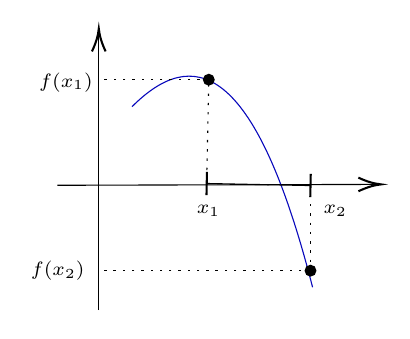
\begin{tikzpicture}[x=0.75pt,y=0.75pt,yscale=-1,xscale=1]
%uncomment if require: \path (0,300); %set diagram left start at 0, and has height of 300

%Straight Lines [id:da014135415149278518] 
\draw    (38,81) -- (192,80.58) ;
\draw [shift={(194,80.57)}, rotate = 179.84] [color={rgb, 255:red, 0; green, 0; blue, 0 }  ][line width=0.75]    (10.93,-3.29) .. controls (6.95,-1.4) and (3.31,-0.3) .. (0,0) .. controls (3.31,0.3) and (6.95,1.4) .. (10.93,3.29)   ;
%Straight Lines [id:da0773649335749016] 
\draw    (58,141.14) -- (58,7.57) ;
\draw [shift={(58,5.57)}, rotate = 90] [color={rgb, 255:red, 0; green, 0; blue, 0 }  ][line width=0.75]    (10.93,-3.29) .. controls (6.95,-1.4) and (3.31,-0.3) .. (0,0) .. controls (3.31,0.3) and (6.95,1.4) .. (10.93,3.29)   ;
%Curve Lines [id:da9774163490841201] 
\draw [color={rgb, 255:red, 9; green, 9; blue, 188 }  ,draw opacity=1 ]   (74,43.14) .. controls (103,14.14) and (133,20.71) .. (161,130.14) ;
%Straight Lines [id:da21016871346893207] 
\draw    (110,80.14) -- (160,81.14) ;
\draw [shift={(160,81.14)}, rotate = 181.15] [color={rgb, 255:red, 0; green, 0; blue, 0 }  ][line width=0.75]    (0,5.59) -- (0,-5.59)   ;
\draw [shift={(110,80.14)}, rotate = 181.15] [color={rgb, 255:red, 0; green, 0; blue, 0 }  ][line width=0.75]    (0,5.59) -- (0,-5.59)   ;
%Straight Lines [id:da13352259104694464] 
\draw  [dash pattern={on 0.84pt off 2.51pt}]  (110,78.14) -- (111,30.14) ;
\draw [shift={(111,30.14)}, rotate = 271.19] [color={rgb, 255:red, 0; green, 0; blue, 0 }  ][fill={rgb, 255:red, 0; green, 0; blue, 0 }  ][line width=0.75]      (0, 0) circle [x radius= 2.34, y radius= 2.34]   ;
%Straight Lines [id:da6938519303014277] 
\draw  [dash pattern={on 0.84pt off 2.51pt}]  (160,81.14) -- (160,122.14) ;
\draw [shift={(160,122.14)}, rotate = 90] [color={rgb, 255:red, 0; green, 0; blue, 0 }  ][fill={rgb, 255:red, 0; green, 0; blue, 0 }  ][line width=0.75]      (0, 0) circle [x radius= 2.34, y radius= 2.34]   ;
%Straight Lines [id:da4956622413927716] 
\draw  [dash pattern={on 0.84pt off 2.51pt}]  (160,122.14) -- (58,122.14) ;
%Straight Lines [id:da37563315618928184] 
\draw  [dash pattern={on 0.84pt off 2.51pt}]  (111,30.14) -- (58,30.14) ;

% Text Node
\draw (104,89.4) node [anchor=north west][inner sep=0.75pt]  [font=\scriptsize]  {$x_{1}$};
% Text Node
\draw (165,89.4) node [anchor=north west][inner sep=0.75pt]  [font=\scriptsize]  {$x_{2}$};
% Text Node
\draw (24,116.4) node [anchor=north west][inner sep=0.75pt]  [font=\scriptsize]  {$f( x_{2})$};
% Text Node
\draw (28,25.4) node [anchor=north west][inner sep=0.75pt]  [font=\scriptsize]  {$f( x_{1})$};
\end{tikzpicture}
\caption{Teorema do Valor intermediário e o cálculo de raizes} \label{fig:intermediario}
\end{minipage}
\end{figure}

para usar o método de bissecção para encontrar uma raiz, comece com um palpite para um valor maior que o da raiz e um valor maior que o da raiz. Eles não precisam ser palpites exatos, ou mesmo particularmente bons palpites, mas eles têm que estar em ambos os lados da raiz. Nós vamos chamar o palpite à esquerda da raiz de $x_1$ e o palpite à direita da raiz $x_2$, ou seja a raiz deve estar no intervalo $(x_1, x_2)$. Em seguida, calculamos o ponto médio deste intervalor $m = \frac{x_2 - x_1}{2}$. Compare os sinais de $f(m)$ e $f(x_1)$: se os sinais forem diferentes, então a raiz deve estar entre $x_1$ e $m$, então fazemos $x_2 = m$. Se os sinais forem os mesmos, então o raiz deve estar entre $m$ e $x_2$, então fazemos $x_1 = m$. Agora temos dois novos palpites $x_1$ e $x_2$ tais que raiz ainda está entre os dois, mas eles estão a metade da distância! Podemos repetir esse processo até que a distância entre $x_1$ e $x_2$ seja menor que a precisão desejada para o cálculo da raiz. O código abaixo implementa este método.

\begin{lstlisting}[language=Python, frame=lines,basicstyle=\footnotesize, caption={Método da Bisecção para cálculo de raizes}, label={lst:bisection}]
def root_bissection (f, x1, x2, tolerance=10e-6):
    dx = np.abs(x2-x1)/2
    while dx > tolerance:
        m = (x2+x1)/2 
        if f(x1)*f(m) < 0:
            x2 = m
        else:
            x1 = m
        dx = np.abs(x2-x1)/2
    return (x2+x1)/2
\end{lstlisting}

Podemos agora usar a função acima para calcular uma raiz de
\[e^x \ln x - x^2 = 0 \]
Veja que fazendo $f(x) = e^x \ln x - x^2$, temos $f(1)=e-1 > 0$ enquanto $f(2)= e^2 \ln 2 - 4<0$, de forma que temos uma raiz no intervalo $(1,2)$. Vamos procurar uma raiz com uma precisão maior que $10^{-7}$. O código abaixo retornará o valor $1.6946001052856445$
\begin{lstlisting}
def f(x):
    return np.exp(x)*np.log(x)-x**2
    
root_bissection(f, 1, 2)
\end{lstlisting}

\subsection{Método de Newton-Raphson}
    
Vamos admitir que a função $f$ que estamos interessados seja contínua e tenha uma derivada contínua em torno da da raiz $r$. O método de Newton-Raphson requer que se conheça tanto a função quanto a derivada da mesma. A idéia básica esta ilustrada na Fig. \ref{fig:Newton_method}

\begin{figure}
\centering
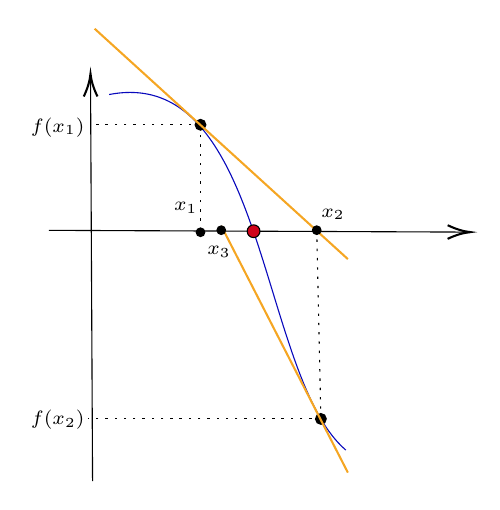
\begin{tikzpicture}[x=0.75pt,y=0.75pt,yscale=-1,xscale=1]
%uncomment if require: \path (0,300); %set diagram left start at 0, and has height of 300

%Straight Lines [id:da6341696579970126] 
\draw    (53,137) -- (254,137.85) ;
\draw [shift={(256,137.86)}, rotate = 180.24] [color={rgb, 255:red, 0; green, 0; blue, 0 }  ][line width=0.75]    (10.93,-3.29) .. controls (6.95,-1.4) and (3.31,-0.3) .. (0,0) .. controls (3.31,0.3) and (6.95,1.4) .. (10.93,3.29)   ;
%Straight Lines [id:da9386272492750976] 
\draw    (74,257.86) -- (73.01,63.57) ;
\draw [shift={(73,61.57)}, rotate = 89.71] [color={rgb, 255:red, 0; green, 0; blue, 0 }  ][line width=0.75]    (10.93,-3.29) .. controls (6.95,-1.4) and (3.31,-0.3) .. (0,0) .. controls (3.31,0.3) and (6.95,1.4) .. (10.93,3.29)   ;
%Curve Lines [id:da7332771912501077] 
\draw [color={rgb, 255:red, 9; green, 9; blue, 188 }  ,draw opacity=1 ]   (82,71.57) .. controls (158,56.86) and (154,206.86) .. (196,242.86) ;
%Straight Lines [id:da6694568846719067] 
\draw  [dash pattern={on 0.84pt off 2.51pt}]  (126,136.86) -- (126,86.14) ;
\draw [shift={(126,86.14)}, rotate = 270] [color={rgb, 255:red, 0; green, 0; blue, 0 }  ][fill={rgb, 255:red, 0; green, 0; blue, 0 }  ][line width=0.75]      (0, 0) circle [x radius= 2.34, y radius= 2.34]   ;
%Straight Lines [id:da32648674551759416] 
\draw  [dash pattern={on 0.84pt off 2.51pt}]  (126,86.14) -- (73,86.14) ;
%Shape: Circle [id:dp5859673038412545] 
\draw  [fill={rgb, 255:red, 208; green, 2; blue, 27 }  ,fill opacity=1 ] (148.5,137.43) .. controls (148.5,135.73) and (149.88,134.36) .. (151.57,134.36) .. controls (153.27,134.36) and (154.64,135.73) .. (154.64,137.43) .. controls (154.64,139.12) and (153.27,140.5) .. (151.57,140.5) .. controls (149.88,140.5) and (148.5,139.12) .. (148.5,137.43) -- cycle ;
%Straight Lines [id:da10660529376202699] 
\draw [color={rgb, 255:red, 245; green, 166; blue, 35 }  ,draw opacity=1 ][line width=0.75]    (75,39.86) -- (197,150.86) ;
%Shape: Circle [id:dp40229126767091916] 
\draw  [fill={rgb, 255:red, 0; green, 0; blue, 0 }  ,fill opacity=1 ] (123.93,137.93) .. controls (123.93,136.78) and (124.86,135.86) .. (126,135.86) .. controls (127.14,135.86) and (128.07,136.78) .. (128.07,137.93) .. controls (128.07,139.07) and (127.14,140) .. (126,140) .. controls (124.86,140) and (123.93,139.07) .. (123.93,137.93) -- cycle ;
%Shape: Circle [id:dp3954498218929916] 
\draw  [fill={rgb, 255:red, 0; green, 0; blue, 0 }  ,fill opacity=1 ] (179.93,136.93) .. controls (179.93,135.78) and (180.86,134.86) .. (182,134.86) .. controls (183.14,134.86) and (184.07,135.78) .. (184.07,136.93) .. controls (184.07,138.07) and (183.14,139) .. (182,139) .. controls (180.86,139) and (179.93,138.07) .. (179.93,136.93) -- cycle ;
%Straight Lines [id:da6934090507517374] 
\draw  [dash pattern={on 0.84pt off 2.51pt}]  (182,136.93) -- (184,227.86) ;
\draw [shift={(184,227.86)}, rotate = 88.74] [color={rgb, 255:red, 0; green, 0; blue, 0 }  ][fill={rgb, 255:red, 0; green, 0; blue, 0 }  ][line width=0.75]      (0, 0) circle [x radius= 2.34, y radius= 2.34]   ;
%Straight Lines [id:da1537553578982449] 
\draw  [dash pattern={on 0.84pt off 2.51pt}]  (184,227.86) -- (72,227.86) ;
%Straight Lines [id:da37580887976486443] 
\draw [color={rgb, 255:red, 245; green, 166; blue, 35 }  ,draw opacity=1 ][line width=0.75]    (136,134.86) -- (197,253.71) ;
%Shape: Circle [id:dp2674385235762444] 
\draw  [fill={rgb, 255:red, 0; green, 0; blue, 0 }  ,fill opacity=1 ] (133.93,136.93) .. controls (133.93,135.78) and (134.86,134.86) .. (136,134.86) .. controls (137.14,134.86) and (138.07,135.78) .. (138.07,136.93) .. controls (138.07,138.07) and (137.14,139) .. (136,139) .. controls (134.86,139) and (133.93,138.07) .. (133.93,136.93) -- cycle ;

% Text Node
\draw (112,122.4) node [anchor=north west][inner sep=0.75pt]  [font=\scriptsize]  {$x_{1}$};
% Text Node
\draw (43,81.4) node [anchor=north west][inner sep=0.75pt]  [font=\scriptsize]  {$f( x_{1})$};
% Text Node
\draw (183,125.4) node [anchor=north west][inner sep=0.75pt]  [font=\scriptsize]  {$x_{2}$};
% Text Node
\draw (43,222.4) node [anchor=north west][inner sep=0.75pt]  [font=\scriptsize]  {$f( x_{2})$};
% Text Node
\draw (128,143.4) node [anchor=north west][inner sep=0.75pt]  [font=\scriptsize]  {$x_{3}$};


\end{tikzpicture}

\caption{Método de Newton para encontrar uma raiz. Com uma estimativa inicial $x_1$, o
valor da função de sua inclinação em $x_1$, o método nos fornece a próxima aproximação
$x_2$. O valor da função e a inclinação em $x_2$ leva para a aproximação $x_3$, e assim sucessivamente até que se atinja a tolerância desejada} \label{fig:Newton_method}
\end{figure}
Conforme a Fig. \ref{fig:Newton_method}, se temos uma aproximação $x_n$ a aproximação seguinte, $x_{n+1}$, será dada pela intersecção da reta tangente a função $f$ em $x_n$ e o eixo $x$, ou seja satisfaz
\[f'(x_n)x_{n+1}+(f(x_n)-f'(x_n)x_n) = 0 \]
e portanto
\[x_{n+1} = x_n - \frac{f(x_n)}{f'(x_n)}.\]
Vale notar que $r$ é um ponto fixo desta sequência, i.e. 
\[ r = r - \frac{f(r)}{f'(r)}.\]
Note também que 
\[\left| x_{n+1} - x_n \right| = \left|\frac{f(x_n)}{f'(x_n)}\right| \]
e portanto a medida que $f(x_n)$ se aproxima de 0 as aproximações ficarão cada vez mais próximas. É claro que há uma dificuldade quando a raiz $r$ não for simples, pois neste caso $f'(r)=0$. 

\begin{lstlisting}[language=Python, frame=lines,basicstyle=\footnotesize, caption={Método da Newton-Raphson para cálculo de raizes}, label={lst:met-newton}]
def root_newton (f,df, x1, tolerance=10e-6):
    x = x1
    dx = 2*tolerance 
    while dx > tolerance:
        xa = x
        x += -f(x)/df(x)
        dx = np.abs(x-xa)
    return x 
\end{lstlisting}

Em geral o método de Newton é muito mais rápido que o método da bissecção. No entanto, como vimos ele possui vários problemas. O palpite inicial deve ser próximo da solução real, e em torno das raiz não deve haver nenhum pronto crítico (onde $f'(x)=0$). É claro que o método de Newton não funciona bem perto de descontinuidades em $f$. Além disso uma desvantagem obvia é que este método requer conhecimento de $f'(x)$. Se você não sabe, ou não pode obter,
uma função que descreve a derivada, então o método de Newton não é uma opção.

\subsection{Método da Secante}

O método da secante é uma variação do método de Newton que não requer o conhecimento explicito do valor da derivada da função. A ideia é iniciar com dois palpites próximos $x_1$ e $x_2$ e utiliza-los para aproximar 

\section{Diferenciação Numérica}

Vamos discutir nessa seção estratégias numéricas para aproximação de derivadas de funções reais. Nosso objetivo é calcular aproximadamente a derivada de uma função a partir de um conjunto de pontos discretos $\{(x_i,y_i)\}_{i=0}^n$. Começamos discutindo as chamadas aproximações por diferenças finitas e, então, as aproximações de derivadas via ajuste ou interpolação. 

Começamos com a fórmula mais simples que pode ser obtida do cálculo diferencial. Seja  uma função diferenciável $f: (a,b) \to \mathbb{R}$. A derivada de $f$  no ponto $x_0 \in (a,b)$  é, por definição,
\[ \frac{\dd }{\dd x} f(x_0) = \lim_{\delta \to 0} \frac{f(x_0+\delta) - f(x_0)}{\delta}.\]
Para aproximar a derivada podemos tomar $\delta > 0$ muito pequeno\footnote{Mesmo pequeno  $\delta$ ainda precisa ser muito maior do que a precisão de float-point, na verdade muito maior que a precisão númerica para o cálculo de $f(x)$, caso contrário corremos riscos de cancelamentos catastróficos.} e obter a aproximação:
\[\frac{\dd }{\dd x} f(x_0) \approx D^+_\delta f (x_0) = \frac{f(x_0+\delta) - f(x_0)}{\delta}  \]
que é chamada de {\it diferença finita progressiva de ordem 1}. De maneira similar temos a {\it diferença finita regressiva de ordem 1}, tomando $h<0$, ou de maneira análoga com $\delta>0$
\[\frac{\dd }{\dd x} f(x_0) \approx D^-_\delta f (x_0) = \frac{f(x_0) - f(x_0 - \delta)}{x_0}. \]
A existência da derivada de $f$ em $x_0$ garante que as duas aproximações tendam a um mesmo valor conforme $\delta \to 0$, i.e. 
\[ \lim_{\delta \to 0} |D_\delta^+ f(x_0) - D_\delta^- f(x_0) |= 0 \]

Vamos observar essa propriedade com a função cosseno em $\frac{\pi}{4}$ usando os valores
$\delta = 0.1, 10^{-2}, 10^{-3}, 10^{-4}$. 

\begin{lstlisting}[language = Python]
import numpy as np

def forward_dif(func, x, h):
    return (func(x+h) - func(x))/h

def regressive_dif(func, x, h):
    return (func(x) - func(x-h))/h

x =  np.pi/4
diferences = np.zeros(5)
h_list = [0.1, 0.01, 0.001, 0.0001, 0.00001]
for i,h in enumerate(h_list):
    diferences[i] = (forward_dif(np.cos, x , h)
                     - regressive_dif(np.cos, x , h))

print(diferences)
\end{lstlisting}

{\bf Exercício} adapte o código acima para calcular quão próximo estamos do valor correto da derivada de $\cos x$

Se $f$ for uma função analítica a obtenção de aproximações para derivadas é um consequência 
da expansão em série de Taylor
\[ f(x_0+\delta) = \sum_{k=1}^{+\infty} \frac{\dd^k}{\dd x^k}f(x_0) \frac{\delta^k}{k!},\]
onde $\frac{\dd^{0}}{\dd x^{0}} f(x_0) \equiv f(x_0)$. O erro ao truncarmos a expansão em um expoente $k=n+1$ é da ordem de $\delta^{n+1}$, mais precisamente
\[ f(x_0+\delta) = f(x_0) + \frac{\dd}{\dd x} f(x_0)\delta + \frac{\dd^2}{\dd x^2}f(x_0) \frac{\delta^2}{2} + \cdots + \frac{\dd^{k+1}}{\dd x^{k+1}}f(x_0) \frac{\delta^{k+1}}{n!}+\frac{\dd^k}{\dd x^k}f(\eta) \frac{\delta^k}{k!},\]
onde $\eta \in [x, x+\delta]$. Ou seja, nossa aproximação por diferenças finitas em primeira ordem possui um erro da ordem de $\delta^2$ (compare com o resultado do código acima). Podemos obter uma melhor aproximação fazendo um {\it diferença finita central}. Note que que
\[\begin{array}{rcl}
f(x_0+\delta) & = & f(x_0) + \frac{\dd}{\dd x}f(x_0) \delta + \frac{\dd^2}{\dd x^2}f(x_0)  \frac{\delta^2}{2!}+ \mathcal{O}(\delta^3)\\
f(x_0-\delta) & = & f(x_0) - \frac{\dd}{\dd x}f(x_0) \delta + \frac{\dd^2}{\dd x^2}f(x_0)  \frac{\delta^2}{2!}+ \mathcal{O}(\delta^3)
\end{array}\]
Temos portanto
\[f(x_0+\delta) - f(x_0-\delta) = 2 \frac{\dd}{\dd x}f(x_0) \delta + \mathcal{O}(\delta^3).\]
Com isso podemos adotar a aproximação
\[\frac{\dd }{\dd x} f(x_0) \approx D_\delta f (x_0) = \frac{f(x_0+\delta) - f(x_0-\delta)}{\delta}.\]

{\bf Exercício:} Mostre que $D_\delta f = D^+_\delta f - D^-_\delta f$

O exemplo abaixo utilizará as funções \lstinline{forward_dif} e \lstinline{regressive_dif} do exemplo anterior para compara os erros nas aproximações das derivadas de $f(x) = e^{e^x}$ em $x = 0$. O cálculo exato nos fornece (fazendo $u=e^x$)
\[f'(x) = \left.\frac{\dd e^u}{\dd u}\right|_{u=e^x} \left.\frac{\dd u}{\dd x}\right|_{x=0} = \left. e^{e^x}e^x \right|_{x=0} = e \]

\begin{lstlisting}[language = Python]
def center_dif(func, x, h):
    return (func(x+h) - func(x-h))/(2*h)

def exp_exp(x):
    return np.exp(np.exp(x))

e = np.exp(1)
Error_f = np.zeros(5)
Error_r = np.zeros(5)
Error_c = np.zeros(5)

h_list = [0.1, 0.01, 0.001, 0.0001, 0.00001]
for i,h in enumerate(h_list):
    Error_f[i] =  e - forward_dif(exp_exp, 0, h_list[i])
    Error_r[i] =  e - regressive_dif(exp_exp, 0, h_list[i])
    Error_c[i] = e - center_dif(exp_exp, 0, h_list[i])

print('Erro Progressivo=', Error_f, 'Erro regressivo', Error_r, 
    'Erro_central =', Error_c)
\end{lstlisting}

A série de Taylor também nos permite obter uma aproximação para a deriva segunda. Novamente
note que que
\[\begin{array}{rcl}
f(x_0+\delta) & = & f(x_0) + \frac{\dd}{\dd x}f(x_0) \delta + \frac{\dd^2}{\dd x^2}f(x_0)  \frac{\delta^2}{2!}+ \mathcal{O}(\delta^3)\\
f(x_0-\delta) & = & f(x_0) - \frac{\dd}{\dd x}f(x_0) \delta + \frac{\dd^2}{\dd x^2}f(x_0)  \frac{\delta^2}{2!}+ \mathcal{O}(\delta^3)
\end{array}\]
Temos portanto
\[f(x_0+\delta) + f(x_0-\delta) = 2 f(x_0) + \frac{\dd^2}{\dd x^2}f(x_0) +  \mathcal{O}(\delta^3).\]
E portanto podemos adotar a aproximação (com um erro da ordem de $\delta^2$)
\[\frac{\dd^2}{\dd x^2}f(x_0) \approx D_\delta^2 f(x_0) = \frac{f(x_0+\delta) + f(x_0-\delta) - 2 f(x_0)}{\delta^2}.\]

Vale destacar que existem outros métodos para aproximação de derivadas de uma função.

\subsection{Erros de Arredondamento}





\section{Integração Numérica}

\section{Equações Diferenciais Ordinárias}

Nessa Seção, vamos discutir métodos numéricos para aproximar a solução de problemas de valor inicial para equações diferenciais ordinárias. Com efeito toda a mecânica é um problema deste tipo. Por exemplo, considere uma força $F(x,\dot x, t)$ agindo em partícula que em $t=0$ esta na posição $x(0)=x_0$ e com velocidade $\dot x(0) = v_0$. Encontrar a posição e velocidade da partícula em um tempo $t>0$, consiste em encontrar uma função $x(t)$ que obedeça a equação diferencial de segunda ordem
\[ \ddot x = F(x,\dot x, t)\]
e satisfaça as condições iniciais $x(0)=x_0, \dot x(0) = v_0$.

Comecemos pelos problemas de primeira ordem e, depois, mostraremos que estas técnicas podem ser estendidas para problemas e sistemas de ordem superior. Considere um problema de valor inicial de primeira ordem dado por:

\begin{equation}\label{eq:1storderODE}\begin{array}{rcl}
\dot x(t) & = & f(x , t),\,\,\, t>0\\
x(t_0) & = & x_0
\end{array}\end{equation}

Vamos explorar como obter uma solução numérica para este problema. Vamos considerar inicialmente um método de passo único conhecido como método de Euler.

\subsection{Método de Euler}

Este é o método mais básico para integração numérica de equações diferenciais ordinárias. A ideia do método consiste em fixas um passo adequadamente pequeno $\Delta t$ e fazer a aproximação 
\[ \frac{\dd x(t)}{\dd t} \approx \frac{x(t+\Delta t) - x(t)}{\Delta t}\]
Dessa forma a eq \ref{eq:1storderODE} pode ser aproximada por
\begin{equation}\label{eq:Euler-Method}\begin{array}{rcl}
x(t + \Delta t) & = & x(t) + f(x , t) \Delta t + \mathcal{O}(\Delta t^2),\,\,\, t>0\\
x(t_0) & = & x_0.
\end{array}\end{equation}
Note que o erro da aproximação é da ordem de $\Delta t^2$.

Isso nos permite criar arrays com $N+1$ entradas
\[\begin{array}{rcl}
    t &=& [t_0, t_1, t_2, \cdots, t_N ] \\
    x &=& [x_0, x_1, x_2, \cdots, x_N ]
\end{array} \]
onde 
\[ t_{i+1} = t_i + \Delta t, \,\,\, x_{i+1} = x_i + f(x,t)\Delta t \]
e o passo $\Delta t = \left|\frac{t_N - t_0}{N} \right|$.

{\bf Exemplo:} Como um exemplo vamos considerar o caso 
\[\begin{array}{rcl}
\dot x(t) & = & x(t),\,\,\, t>0\\
x(0) & = & 1
\end{array}\]
Este problema tem uma solução analítica simples dada por $x(t)=e^{t}$ que pode ser verificada diretamente por substituição na EDO acima. 

\begin{lstlisting}[language = Python]
import numpy as np
import matplotlib.pyplot as plt

tempo_0 = 0
tempo_f = 1
x_0 = 1
passos = 1000
dt = (tempo_f - tempo_0)/passos
t_list = np.zeros(passos)
x_list = np.zeros(passos)

#Condicoes iniciais
t_list[0] = tempo_0
x_list[0] = x_0

for i in range(passos-1):
    t_list[i+1] =  t_list[i]+dt
    x_list[i+1] = x_list[i]*(1+dt)

plt.scatter(t_list, x_list, label='Metodo de Euler', marker='+')
plt.plot(t_list, np.exp(t_list), 
    label='Resultado Analitico', color='red')
plt.legend()
plt.show()
print('Tamanho do passo=', dt, 'Erro Maximo =', 
    np.abs((x_list-np.exp(t_list))).max())
\end{lstlisting}

Varie o tamanho do passo e note oque acontece com o erro.

{\bf Exemplo:} Vamos considerar agora o caso
\[\begin{array}{rcl}
\dot x(t) & = & \cos t,\,\,\, t>0\\
x(0) & = & 0
\end{array}\]
É fácil ver que a solução deste problema é dada por $x(t) = \sin t$. Nesse exemplo vemos como a ordem de escolha do valor de $t$ para o update da posição $x$ é relevante. Note que temos duas formas:
\[ x(t+dt) \approx x(t) = dt*\cos t,\,\, \textrm{e} \,\,\,x(t+dt) \approx x(t) = dt*\cos (t+dt)\]

Na primeira utilizamos o valor anterior de $t$ para o cálculo da derivada e enquanto no segundo caso utilizamos o valor $t+dt$ para o cálculo da derivada. A saída deve ser como a mostrada na \ref{fig:euler2}.


\begin{lstlisting}[language = Python]
import numpy as np
import matplotlib.pyplot as plt

tempo_0 = 0
tempo_f = 3
x_0 = 0
passos = 100
dt = (tempo_f - tempo_0)/passos
t_list = np.zeros(passos)
x_list = np.zeros(passos)
x_list1 = np.zeros(passos)

#Condicoes iniciais
t_list[0] = tempo_0
x_list[0] = x_0

for i in range(passos-1):
    t_list[i+1] =  t_list[i]+dt
    x_list[i+1] = x_list[i]+np.cos(t_list[i])*dt
    x_list1[i+1] = x_list1[i]+np.cos(t_list[i+1])*dt

plt.scatter(t_list, x_list, 
    label='Metodo de Euler update c\ t anterior', marker='+', s=1)
plt.scatter(t_list, x_list1,
    label='Metodo de Euler update c\ t atual', marker='o', s=1)
plt.plot(t_list, np.sin(t_list), label='Solucao Analitica',
    color='red', linewidth=0.5)
plt.legend()
plt.show()
print('Tamanho do passo=', dt, 'Erro Maximo (t anterior)=',
    np.abs((x_list-np.sin(t_list))).max(),Erro Maximo (t atual)=',
    np.abs((x_list1-np.sin(t_list))).max())
\end{lstlisting}



\begin{figure}
    \centering
    \includegraphics{Images/euler2.png}
    \caption{Método de Euler progressivo e Regressivo}
    \label{fig:euler2}
\end{figure}

\subsection{Variações do Método de Euler}
\subsection{Método de Runge-Kutta}
\section{Método de Monte Carlos}\label{sc:Monte_Carlo}
\section{Métodos Estocásticos}
\section{Equações Diferenciais Parciais}
\subsection{Equação de Laplace}
\subsection{Equação da Onda}
\subsection{Equação do Calor}
